% Configuración del documento y paquetes
\documentclass[12pt,a4paper]{article}
\usepackage[english,spanish]{babel}
\usepackage[utf8]{inputenc}
\usepackage[T1]{fontenc}
\usepackage{amsmath}
\usepackage{svg}
\usepackage{graphicx}
\usepackage[colorinlistoftodos]{todonotes}
\usepackage[top=1.5cm, bottom=2.0cm, left=1.50cm, right=1.50cm]{geometry}
\usepackage[nottoc]{tocbibind}
\usepackage{amssymb}
\usepackage{hyperref}
\usepackage{textcomp}
\usepackage{multicol} 
\usepackage{longtable} 
\usepackage[printonlyused,withpage]{acronym}
\usepackage[justification=centering]{caption}
\usepackage{afterpage}
\usepackage{subfig}
\usepackage[export]{adjustbox}
\usepackage{float}

\usepackage{appendix}
\renewcommand{\appendixname}{Anexos}
\renewcommand{\appendixtocname}{Anexos}
\renewcommand{\appendixpagename}{Anexos}

\usepackage{listings}
\usepackage{color}
\definecolor{codegreen}{rgb}{0,0.6,0}
\definecolor{codegray}{rgb}{0.5,0.5,0.5}
\definecolor{codepurple}{rgb}{0.58,0,0.82}
\definecolor{backcolour}{rgb}{0.95,0.95,0.92}
\definecolor{gray75}{gray}{.75}
\lstdefinestyle{mystyle}{
    backgroundcolor=\color{backcolour},   
    commentstyle=\color{codegreen},
    keywordstyle=\color{magenta},
    numberstyle=\tiny\color{codegray},
    stringstyle=\color{codepurple},
    basicstyle=\footnotesize,
    breakatwhitespace=false,         
    breaklines=true,                 
    captionpos=b,                    
    keepspaces=true,                 
    numbers=left,                    
    numbersep=5pt,                  
    showspaces=false,                
    showstringspaces=false,
    showtabs=false,                  
    tabsize=2,
    literate=
  {á}{{\'a}}1 {é}{{\'e}}1 {í}{{\'i}}1 {ó}{{\'o}}1 {ú}{{\'u}}1
  {Á}{{\'A}}1 {É}{{\'E}}1 {Í}{{\'I}}1 {Ó}{{\'O}}1 {Ú}{{\'U}}1
  {à}{{\`a}}1 {è}{{\`e}}1 {ì}{{\`i}}1 {ò}{{\`o}}1 {ù}{{\`u}}1
  {À}{{\`A}}1 {È}{{\'E}}1 {Ì}{{\`I}}1 {Ò}{{\`O}}1 {Ù}{{\`U}}1
  {ä}{{\"a}}1 {ë}{{\"e}}1 {ï}{{\"i}}1 {ö}{{\"o}}1 {ü}{{\"u}}1
  {Ä}{{\"A}}1 {Ë}{{\"E}}1 {Ï}{{\"I}}1 {Ö}{{\"O}}1 {Ü}{{\"U}}1
  {â}{{\^a}}1 {ê}{{\^e}}1 {î}{{\^i}}1 {ô}{{\^o}}1 {û}{{\^u}}1
  {Â}{{\^A}}1 {Ê}{{\^E}}1 {Î}{{\^I}}1 {Ô}{{\^O}}1 {Û}{{\^U}}1
  {œ}{{\oe}}1 {Œ}{{\OE}}1 {æ}{{\ae}}1 {Æ}{{\AE}}1 {ß}{{\ss}}1
  {ű}{{\H{u}}}1 {Ű}{{\H{U}}}1 {ő}{{\H{o}}}1 {Ő}{{\H{O}}}1
  {ç}{{\c c}}1 {Ç}{{\c C}}1 {ø}{{\o}}1 {å}{{\r a}}1 {Å}{{\r A}}1
  {€}{{\euro}}1 {£}{{\pounds}}1 {«}{{\guillemotleft}}1
  {»}{{\guillemotright}}1 {ñ}{{\~n}}1 {Ñ}{{\~N}}1 {¿}{{?`}}1
}
\renewcommand{\lstlistingname}{Listado}
\lstset{style=mystyle}

\definecolor{maroon}{rgb}{0.5,0,0}
\definecolor{darkgreen}{rgb}{0,0.5,0}
\lstdefinelanguage{XML}
{
  %basicstyle=\ttfamily,
  morestring=[s]{"}{"},
  morecomment=[s]{?}{?},
  morecomment=[s]{!--}{--},
  commentstyle=\color{darkgreen},
  moredelim=[s][\color{black}]{>}{<},
  moredelim=[s][\color{red}]{\ }{=},
  stringstyle=\color{blue},
  identifierstyle=\color{maroon}
}

% Configuración de los márgenes del documento
\usepackage{vmargin}
\setpapersize{A4}
\setmargins{2.5cm} % margen izquierdo
{1.5cm}            % margen superior
{16.6cm}           % anchura del texto
{23.42cm}          % altura del texto
{16pt}             % altura de los encabezados
{1cm}              % espacio entre el texto y los encabezados
{0pt}              % altura del pie de página
{2cm}              % espacio entre el texto y el pie de página

% Configuración de cabecera y pie de página
\usepackage{fancyhdr}
\pagestyle{fancy}
\fancyhf{}
\fancyhead[L]{\nouppercase{\leftmark}}
\fancyfoot[C]{Página \thepage}
\renewcommand{\headrulewidth}{0.5pt}
\renewcommand{\footrulewidth}{0.5pt}
\hypersetup{
    colorlinks=true,
    linkcolor=black,
    filecolor=magenta,      
    urlcolor=blue,
    linkbordercolor=white
}
% diccionario de acrónimos
\usepackage[acronym,toc,shortcuts]{glossaries}
\setlength{\glsdescwidth}{0.8\textwidth}
\makeglossaries
\newacronym{GFLOPS}{GFLOPS}{Giga Floating Point Operations Per Second}
\newacronym{TFLOPS}{TFLOPS}{Tera Floating Operations Per Second}
%\newacronym{}{}{}

% Algoritmos en pseudcódigo 
\usepackage[ruled,linesnumbered,spanish,onelanguage]{algorithm2e}
\SetAlFnt{\footnotesize}
% nuevos comandos (macros)
\newcommand{\seccion}[1]{
\textcolor{blue}{
\hrule height 1.5pt
\section{#1}
\hrule height 1.5pt
\vspace{0.5cm}}
}
\newcommand{\subseccion}[1]{
\textcolor{blue}{\subsection{#1}
\hrule
\vspace{0.5cm}}
}
% Configuración de la portada del documento
\newcommand{\doctitle}{Análisis y clasificación de imágenes médicas mediante redes neuronales}
\newcommand{\docauthor}{Gonzalo Caparrós Laiz}
\newcommand{\docdate}{Junio, 2020}
\newcommand{\docdirector}{Dr. D. Gregorio Bernabé García y Dr. D. José Manuel García Carrasco}

\title{\doctitle}
\author{\docauthor}
\date{\docdate}
% Documento 
\begin{document}
\renewcommand*\listtablename{Índice de tablas}
\renewcommand\spanishtablename{Tabla}
\glsunsetall

\newcommand*{\blankpage}{%
\vspace*{\fill}
{\centering Esta página ha sido intencionadamente dejada en blanco\par}
\vspace{\fill}}
% *********************** Portada del Documento
\begin{titlepage}
\begin{center}
\begin{figure}[ht]
\centering
\includegraphics[width=0.5\textwidth]{img/escudo}
\end{figure}
\vspace{1cm}
\begin{Large}
\textbf{Universidad de Murcia\\
Facultad de Informática\\}
\vspace{0.5cm}
GRADO EN INGENIERÍA INFORMÁTICA\\
\vspace{1.0cm}
\textbf{\doctitle}
\end{Large}
\vspace{1.0cm}
\hrule
\vspace{0.2cm}
\begin{large}
\textbf{Trabajo Fin de Grado realizado por:}\\\docauthor\\
\vspace{0.2cm}
\textbf{Bajo la dirección de:}\\
\docdirector\\
\vspace{0.2cm}
\docdate\\
\end{large}
\vspace{0.5cm}
\hrule
\vspace{1cm}
\end{center}
\end{titlepage}
\pagenumbering{roman}
% *********************** Fin Portada del Documento
\renewcommand{\headrulewidth}{0.0pt}
\renewcommand{\footrulewidth}{0.0pt}
\fancyhead[L]{}
\fancyfoot[C]{}
\newpage
\blankpage
%**************************************************
\newpage
\fancyhead[L]{\nouppercase{\leftmark}}
\fancyfoot[C]{Página \thepage}
\renewcommand{\headrulewidth}{0.5pt}
\renewcommand{\footrulewidth}{0.5pt}
\tableofcontents

\newpage
\listoffigures

\newpage
\listoftables

\newpage
\pagenumbering{arabic}
\section*{Declaración firmada sobre originalidad del trabajo}
\fancyhead[L]{Declaración firmada sobre originalidad del trabajo}
\addcontentsline{toc}{section}{Declaración firmada sobre originalidad del trabajo}

\newpage
\section*{Resumen}
\fancyhead[L]{Resumen}
\addcontentsline{toc}{section}{Resumen}

\newpage
\section*{Extended Abstract}
\fancyhead[L]{Extended Abstract}
\addcontentsline{toc}{section}{Extended Abstract}

\newpage
\section{Introducción}
\fancyhead[L]{\nouppercase{\rightmark}}

Ciertos procedimientos en medicina requieren la dedicación de muchas horas de trabajo de los profesionales del sector, por lo tanto consumen muchos recursos ya sea de tiempo, muy valioso para dar diagnósticos de forma rápida y eficaz, como económicos. Uno de estos procedimientos es el diagnóstico de ciertas enfermedades, los cuales requieren la segmentación de imágenes médicas de distintos órganos y tejidos. En concreto en este trabajo vamos a tratar de la clasificación de las Imágenes por Resonancia Magnética (\textit{MRI}) del corazón y por lo tanto su diagnóstico.
\bigskip

Estas tareas son muy repetitivas siendo esto una ventaja para los programas de inteligencia artificial ya que lo hacen siempre de la misma manera y de forma mucho más rápida que las personas. Este trabajo se basa en el paper \textit{Automatic Segmentation and Disease Classification Using Cardiac Cine MR Images} ~\cite{DBLP:journals/corr/abs-1708-01141} en el que se desarrolla una red neuronal basada en convoluciones dilatadas. En este trabajo se propone una solución al mismo problema pero con un enfoque distinto, partir de una red neuronal ya entrenada en un conjunto de datos distintos y utilizar técnicas de \textit{transfer learning} para resolver el mismo problema que en el paper ~\cite{DBLP:journals/corr/abs-1708-01141}. Se hacen diferentes pruebas y se estudia cual es la mejor solución. En otras palabras se intenta reducir el tiempo de una tarea que hecha por los procedimientos tradicionales sería muy lenta, de esta forma podemos dar un diagnóstico más rápido y a más pacientes. Para llevar a cabo el trabajo se usa el framework \textit{TensorFlow} y se utilizan los modelos de partida que se proporcionan en \textit{TensorFlow Hub}, principalmente \textit{resnet} e \textit{inceptionv3}.

\newpage
\section{Estado del arte}

\subsection{Inteligencia artificial}
Se entiende por inteligencia artificial como los programas que intentan simular el comportamiento humano para resolver un problema. Hay muchos formas de enfocar un programa de inteligencia artificial unas más fáciles de entender como la simbólica, que es un programa basado en reglas que intenta imitar el comportamiento humano, o un enfoque sin símbolos en el que se encontraría el \textit{machine learning}, en el que podemos tener millones de parámetros que entrenar y no saber qué representa cada uno.

\subsection{Machine learning}
Es un tipo de inteligencia artificial sin símbolos que consiste en algoritmos que resuelven un problema sin darle instrucciones explícitas de cómo se resuelve el problema. Estos algoritmos construyen un modelo matemático que suele tener millones de parámetros, que se entrenan, difíciles de analizar para saber qué es lo que hace que dé el resultado que da. Generalmente el \textit{machine learning} se usa para resolver problemas para los que no es factible o es muy difícil hacer un algoritmo tradicional.
\bigskip

Para ello parte de unos datos de muestra o datos de entrada de los que aprenderá a resolver el problema que tiene que resolver, mediante repetición de cálculo del error y ajuste del modelo. Estos datos se suelen dividir en tres conjuntos o sets:

\begin{itemize}
\item \textbf{\textit{Training} set}: este set se usa para que el modelo se entrene. Con este set se calculan los errores en el momento del entrenamiento y se usan para ajustar los parámetros del modelo que se está entrenando.
\item \textbf{\textit{Validation} set}: este set se usa durante el entrenamiento para evaluar el modelo y poder ver el progreso.
\item \textbf{\textit{Test} set}: este set se usa al final, cuando el modelo ya ha sido entrenado, para evaluar el modelo con unos datos que nunca hayan sido vistos de ninguna manera por el modelo.
\end{itemize}

Hay principalmente tres formas de hacer que un modelo aprenda a resolver el problema cada enfoque es más apropiado para resolver un tipo de problema.

\subsubsection{Aprendizaje supervisado}
El aprendizaje supervisado consiste en aplicar \textit{machine learning} a unos datos de entrada que están etiquetados y por lo tanto el modelo aprenderá a etiquetar esas clases. Aplicaciones comunes del aprendizaje supervisado son la clasificacion y regresion. En la clasificación la salida de los modelo es un número limitado de valores que son los que los datos de entrada están etiquetados. En la regresión la salida puede tener cualquier valor numérico en un rango.

\subsubsection{Aprendizaje no supervisado}
El aprendizaje no supervisado consiste en aplicar \textit{machine learning} a unos datos de entrada que no estén etiquetados y el modelo aprenda a encontrar patrones en esos datos y a agruparlos de forma automática.

\subsubsection{Aprendizaje por refuerzo}
El aprendizaje por refuerzo consisten en agentes que se mueven por un entorno realizando acciones obteniendo una recompensa cuando se van acercando a la solución. El objetivo básico es maximizar la recompensa. En este enfoque no es necesario unos datos de entrada etiquetados.

\subsection{Redes Neuronales}
Inspiradas en el funcionamiento de las redes neuronales biológicas, una red neuronal es una forma de organizar los modelos de inteligencia artificial para abordar ciertos problemas que son difíciles de resolver con la programación ordinaria basada en ``Reglas'' obteniendo muy buenos resultados en una amplia variedad de tareas como por ejemplo: la visión por ordenador o el reconocimiento de la voz.
\bigskip

Este tipo de inteligencia artificial se organiza en varias capas interconectadas entre sí. Las capas se suelen nombrar como capa de entrada, que es la primera capa, a la que se le pasan directamente los datos de entrada, capa de salida, que es la última capa, la que da el resultado de la predicción que hace la red neural y capas ocultas, que son las que están entre la primera y la última.
\bigskip

Las capas de una red neuronal están compuestas por neuronas artificiales.

\begin{figure}[H]
\centering
\includegraphics[width=0.3\textwidth]{img/nn}
\caption{Ejemplo de red neuronal con capa de entrada, capa de salida y una capa oculta.}
\end{figure}

\subsubsection{Neuronas artificiales}
Las neuronas artificiales son la unidad básica de una red neuronal reciben una entrada y producen una salida. La entrada la reciben de la capa inmediatamente anterior a la capa a la que pertenecen y la salida es la entrada de la capa inmediatamente a continuación. El funcionamiento básico de una neurona es el siguiente: las entradas se multiplican por un peso y se suman, el valor se le aplica una función que dará la salida de la neurona, también llamada función de activación.

%TODO use minipage
\begin{figure}[H]
\centering
\subfloat{{\large $y_{i} = f\left(\sum_{j=0}^{k}w_{ij}x_{j}\right)$}}%
\qquad
\subfloat{{\includegraphics[valign=c, width=0.3\textwidth]{img/neurona} }}%
\caption{Formula de suma de pesos e imagen de una neurona.}
\end{figure}

%TODO son los pesos que
Donde $f$ es la función de activación, $w_{ij}$ son los pesos, $x_{i}$ son las entradas e $y$ es la salida.
\bigskip

%TODO que es x w 
Algunas de las funciones de activación más usadas son las siguientes. En los siguientes apartados $z$ se refiere a la entrada de la función según la fórmula:
\begin{equation*}
z = \sum_{j=0}^{k} w_{j} x_{j}
\end{equation*}

\begin{itemize}
\item \textbf{Función escalonada}: La salida de esta función es 1 si el valor de entrada es mayor que cierto umbral o 0 si está por debajo del umbral.

\begin{figure}[H]
\centering\begin{minipage}[H]{0.5\textwidth}
\large
\begin{equation*}
y = \begin{cases}
1 & si \: z \geq \alpha \\
0 & si \: z < \alpha
\end{cases}
\end{equation*}
\end{minipage}%
\begin{minipage}[t]{0.5\textwidth}
\includegraphics[valign=c, width=0.8\textwidth]{img/escalonada}
\end{minipage}
\caption{Formula y gráfica.}
\end{figure}
%TODO que es alpha y en este caso alpha es 0

\item \textbf{Combinación lineal}: En esta función la salida simplemente se le suma un bias. Esta función aplica una transformación lineal a la entrada
%TODO formula

\item \textbf{Sigmoide}: Una función sigmoide es una función matemática que tiene la característica que su curva tiene forma de \textit{s}. Con esta función las entradas negativas tienden a cero y conforme la entrada se acerca a cero la salida va aumentando hasta que el valor de entrada es positivo, conforme se aleja de cero tiende a uno. La función más utilizada es la función logística pero otras funciones matemáticas con forma de \textit{s} también se usan como la tangente o la tangente hiperbólica.

\begin{figure}[H]
\centering\begin{minipage}[H]{0.5\textwidth}
\large
\begin{equation*}
y = \frac{1}{1+e^{-x}}
\end{equation*}
\end{minipage}%
\begin{minipage}[t]{0.5\textwidth}
\includegraphics[valign=c, width=0.8\textwidth]{img/sig}
\end{minipage}
\caption{Formula y gráfica.}
\end{figure}
%TODO en este caso se plot la logistica; usar e bien en el plot

\item \textbf{Rectificador}: Esta función se define como la parte positiva de la entrada. Es decir si la entrada es positiva esa es la salida sin embargo si la entrada es negativa la salida es cero.

\begin{figure}[H]
\centering\begin{minipage}[H]{0.5\textwidth}
\large
\begin{equation*}
y = max(0, x)
\end{equation*}
\end{minipage}%
\begin{minipage}[t]{0.5\textwidth}
\includegraphics[valign=c, width=0.8\textwidth]{img/rectificador}
\end{minipage}
\caption{Formula y gráfica.}
\end{figure}

\end{itemize}

\subsubsection{Tipos de capas}
%TODO extender
Hay distintos tipos de capas con diferentes características y funciones.

\begin{itemize}
\item \textbf{Convolución}: Esta capa es de las más usadas y da nombre al tipo de red que se crea. Funciona seleccionando un conjunto de la entrada y combinando los valores en uno solo mediante una función matemática. De esta forma dichos valores se reducen pero el resultado de salida tiene más información comprimida o más significativa. Es como una simplificación.

\begin{figure}[H]
\centering
\includegraphics[width=0.3\textwidth]{img/c}
\caption{Convolución.}
\end{figure}

\item \textbf{Convolución dilatada}: Es una convolución en la que los valores de entrada no se abordan todos juntos sino que se agrupan en círculos, separados por unos espacios, de esta forma los datos de entrada, a cada una de las neuronas de este tipo de capa, abarcan más.

\begin{figure}[H]
\centering
\includegraphics[width=0.3\textwidth]{img/ac}
\caption{Convolución dilatada.}
\end{figure}

\item \textbf{\textit{Pooling}}: Consiste en agrupar los datos en una dimensión usando alguna función matemática. En el caso de \textit{average pool} se usa la media y en el caso de \textit{max pool} el valor máximo.

\begin{figure}[H]
\centering
\includegraphics[width=0.3\textwidth]{img/pool}
\caption{\textit{Pooling}.}
\end{figure}

\item \textbf{Concatenación}: La única función de esta capa es agregar los valores sin hacerles ningún tipo de modificación. No tiene ningún efecto en los resultados.

\item \textbf{\textit{Dropout}}: En esta capa de se modifican aleatoriamente algunos valores asignándoles a su vez a estos otros valores aleatorios. Esto puede parecer contraproducente pero ayuda a reducir el \textit{overfitting}.

\item \textbf{Totalmente conectada}: En esta capa todos las neuronas de la capa anterior están conectadas a todas las neuronas de la capa siguiente. Este tipo de capa se suele poner al final ya que hacer una conexión todos con todos es bastante costoso, pero es la que tiene más potencial para aprender, por estas razones se suelen poner estas capas al final de la red que es donde los tamaños de las capas son más reducidos y la información que proporcionan las capas es más significativa. También esta capa al tener más potencial de aprender también es más propensa a tener \textit{overfitting}, por eso se suele poner antes una capa de \textit{dropout}.

\begin{figure}[H]
\centering
\includegraphics[width=0.3\textwidth]{img/nn}
\caption{Totalmente conectada.}
\end{figure}

\item \textbf{\textit{Softmax}}: Esta capa no hace nada realmente de inteligencia artificial simplemente aplica una fórmula matemática para que todos los valores estén en un rango y con una distribución concreta.

\end{itemize}

\subsubsection{Backpropagation}
Es el proceso en el que se calculan los errores para cada etapa del entrenamiento y según el error se ajustan los pesos de cada capa para reducir el error al maximo. En este proceso se calcula el gradiente de la función \textit{loss} con respecto a los pesos de la red. Uno de los métodos para actualizar los pesos de la red es \textit{stochastic gradient descent}.

\begin{itemize}
\item \textbf{\textit{Stochastic gradient descent}}: Es un método iterativo para optimizar una función objetivo.

\item \textbf{Función \textit{loss}}: Esta función calcula el error entre el resultado de la red neuronal y el resultado correcto que luego se usará en el proceso de \textit{backpropagation} para reajustar los parámetros del modelo que se está entrenando.

\end{itemize}

\subsection{Transfer learning}
La técnica de \textit{transfer learning} consiste en partir de una red neuronal entrenada en un conjunto de datos para resolver un problema y eliminar las últimas capas para reentrenarlas y que resuelvan otro problema. De esta manera se consiguen dos beneficios: se puede entrenar más rápido y con menos recursos y gracias al aprovechamiento del conocimiento adquirido en la red de la que se parte se puede alcanzar una buena precisión con menos recursos.

\subsection{Random forest}
Esta técnica consiste en dividir el problema en varios subproblemas en el caso de la clasificación dividir el conjunto de clases en varios grupos. Y utilizar múltiples modelos de inteligencia artificial para resolver el problema. De esta forma se consigue reducir la dificultad de cada modelo individual y así conseguir más precisión a cambio de incrementar el tiempo de cómputo, ya que hay que entrenar y ejecutar más modelos.

\subsection{Cascada}
Es parecida a \textit{random forest} pero en este caso el problema se divide en tantos como clases tenga la clasificación y la forma de proceder sería la siguiente: el primer modelo distingue entre una clase y el resto, el segundo modelo diferencia entre las clases que quedan y otra clase que no sea la anterior y así sucesivamente hasta que el último modelo tiene que diferenciar entre dos clases.

\subsection{Inception}
Esta arquitectura está basada en \textit{AlexNet}, su objetivo es reducir el coste computacional gracias a la factorización de convoluciones. La forma de esta arquitectura es la siguiente: se divide en bloques de convoluciones. Al principio tiene varias convoluciones una detrás de otra con una capa max \textit{pool} entre medias. Cada uno de los bloques usa la salida del bloque anterior y se pasa como entrada a 4 caminos distintos e independientes uno con una convolución 1x1 otro con convolución 3x3 otro con convolución 5x5 y otro que tiene un \textit{average pool} y una convolución 1x1. Las salidas de los 4 caminos se concatenan y esa será la salida del bloque. Tiene una salida auxiliar que se usará para el entrenamiento. Y al final tiene unas capas de \textit{average pool} seguida de una de \textit{dropout}, una totalmente conectada y finalmente una de \textit{softmax}. La capa totalmente conectada se sitúa al final de la red porque es donde la información está más concentrada y la de \textit{dropout} también porque es donde más posibilidad de \textit{overfitting} hay.

%TODO reduccion de matriz

\subsection{Entrada de datos}
En el campo del \textit{machine learning} un factor muy importante para el éxito del modelo es el conjunto de datos del que se parte, el que representa el problema que se quiere resolver. Uno de los problemas que puede causar un mal conjunto de datos es que no resuelva el problema que queremos o que nos encontremos problemas de \textit{overfitting}. Las características de un buen conjunto de datos son:

\begin{itemize}
\item Las clases de los datos deben de estar en en una proporción igual todos.
\item Al dividir los datos en conjuntos de entrenamiento validación y test tener en cuenta que también hay que mantener la proporción.
\item Si hay datos relacionados entre sí también habrá que tenerlo en cuenta a la hora de hacer la división en los conjuntos de entrenamiento validación y test.

\end{itemize}

\subsubsection{Distorsión}
Consiste en coger el conjunto de datos de entrada y aplicarle algunas transformaciones como por ejemplo en el caso de las imágenes, rotación, traslación o cortes.
\bigskip

Las ventajas de usar distorsión son, aumentar el tamaño del conjunto de datos de entrada, haciendo así posible que ese conjunto de datos sea lo suficientemente grande para poder ser usado. O también otra ventaja es mejorar la calidad de un conjunto de datos con el fin de obtener unos mejores resultados, esto se debe a que al aplicar distorsión la cantidad de posibilidades que el modelo ve se aumenta.

%TODO parrafo en este trabajo ...

\subsubsection{Conjuntos de datos}
Algunos de los conjuntos de datos que hay para entrenar modelos de inteligencia artificial son los siguientes.

\begin{itemize}
\item \textbf{Flores}: Este conjunto de datos está compuesto de aproximadamente 3500 fotos de flores divididas en 5 clases de fotos, cada una aproximadamente 700 fotos. Las imagenes estan en formato comprimido \textit{jpg} y son a color. Las clases son: \textit{daisy}, \textit{dandelion}, \textit{roses}, \textit{sunflowers} y \textit{tulips}.

\begin{figure}[H]
\centering
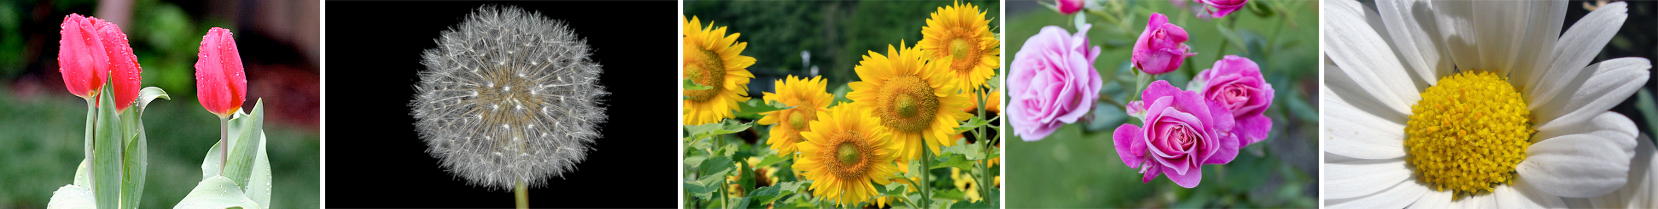
\includegraphics[width=0.3\textwidth]{img/flores}
\caption{Muestra del \textit{dataset} flores.}
\end{figure}

\item \textbf{\textit{ACDC}}: El \textit{dataset} se compone de 150 pacientes reales de los que se les ha sacado unas resonancias magnéticas del corazón las cuales han sido anonimizadas. Las resonancias de los 150 pacientes están divididas en 5 clases (4 enfermedades y una normal). También incluye información adicional del paciente como el peso la altura, y los frames claves de las resonancias. El \textit{dataset} pertenece a un reto (\textit{Automated Cardiac Diagnosis Challenge}) por eso solo se proporciona la segmentación de referencia de 100 pacientes las del resto son parte del reto. Las imagenes estan en escala de grises y el formato es sin compresión. Las clases son: \textit{normal} (\textit{NOR}), \textit{myocardial infarction} (\textit{MINF}), \textit{dilated cardiomyopathy} (\textit{DCM}), \textit{hypertrophic cardiomyopathy} (\textit{HCM}) y \textit{abnormal right ventricle} (\textit{RV}).

\begin{figure}[H]
\centering
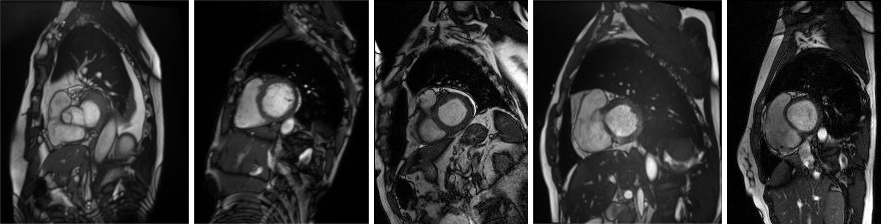
\includegraphics[width=0.3\textwidth]{img/acdc}
\caption{Muestra del \textit{dataset} \textit{ACDC}.}
\end{figure}

%TODO parrafo los datos ...

%TODO apartado imagenet

%TODO apartado cifar 10 100

\end{itemize}

%TODO apartado framework

\newpage
\section{Análisis de objetivos y metodología}
\subsection{Objetivos}
El objetivo de este trabajo es buscar una solución para la clasificación de enfermedades cardiacas en el \textit{dataset} \textit{ACDC} usando \textit{transfer learning} y diferentes enfoques para encontrar la solución que mejores resultados obtenga. Se usa como referencia el paper \textit{Automatic Segmentation and Disease Classification Using Cardiac Cine MR Images} ~\cite{DBLP:journals/corr/abs-1708-01141} en él proponen una solución en la que primero se segmentan las imágenes del corazón y luego se usa un clasificador \textit{random forest} para clasificar la imagen de entrada.
\bigskip

A diferencia del paper ~\cite{DBLP:journals/corr/abs-1708-01141} en el que se diseña una arquitectura específica y se entrena un modelo exclusivamente para ese problema, en este trabajo se parte de arquitecturas y modelos ya desarrollados y entrenados para resolver otro problema y se usa la técnica de \textit{transfer learning} para adaptarlo al nuevo problema.

\subsection{Metodología}
La forma de realizar el trabajo es realizando distintas pruebas de diferentes características para estudiar cuál es la opción más interesante o que obtenga los mejores resultados.

\newpage
\section{Diseño y resolución del trabajo realizado}
En esta sección describo los pasos y las pruebas que he realizado y el proceso que he seguido para llegar a la solución que finalmente he obtenido, que consisten en realizar pruebas con diferentes modelos de partida ver los resultados obtenidos y analizar los resultados.
\bigskip

En estas pruebas todos los modelos de partida que he usado se han obtenido de la herramienta \textit{TensorFlow Hub}, los cuales ya vienen preparados para ser reentrenados para que solucionen otro problema. Todos los modelos han sido entrenados en el \textit{dataset} \textit{ImageNet} con 1000 clases, por lo tanto tienen el suficiente ``conocimiento'' como para resolver otro problema de clasificación menos exigente como por ejemplo la clasificación de 10 clases.

\subsection{Técnica bottleneck}
La técnica de \textit{bottleneck} consiste en obtener primero los valores del \textit{tensor} de salida de todos las imágenes de entrada, y guardar los valores, de esta manera no se tiene que ejecutar toda la red cada vez que vamos a entrenar con cierta imagen. De esta manera se entrena un modelo más pequeño, solamente las últimas capas y se usa como entrada de ese pequeño modelo la salida de toda la parte del modelo que no vamos a entrenar.
\bigskip

En cuanto a la inferencia usando esta técnica no cambia y se realiza de la misma manera que se haría con el resto de modelos que no usen esta técnica.

\begin{figure}[H]
\centering
\subfloat[Entrenamiento]{{\includegraphics[valign=c, width=0.3\textwidth]{example-image} }}%
\qquad
\subfloat[Inferencia]{{\includegraphics[valign=c, width=0.3\textwidth]{example-image} }}%
\caption{Pasos para realizar el entrenamiento usando la técnica de \textit{bottleneck} y para la inferencia.}
\end{figure}

\subsection{Pruebas en otros datasets}
\subsubsection{Entrenamiento completo}
La primera prueba consiste en hacer un entrenamiento completo y así poder comparar los resultados con otras técnicas que voy a usar. En esta prueba se entrena de 0 la arquitectura \textit{AlexNet} para clasificar las imágenes del \textit{dataset} \textit{cifar 10}.

\begin{table}[H]
\centering
\begin{tabular}{|l|l|l|l|l|l|l|}
\hline
\textbf{Modelo} & \textbf{Dataset}              & \textbf{Clases}         & \textbf{Iteraciones}        & \textbf{Learning rate}   & \textbf{Batch size}      & \textbf{Precisión}        \\ \hline
AlexNet         & \multicolumn{1}{c|}{cifar 10} & \multicolumn{1}{c|}{10} & \multicolumn{1}{c|}{100000} & \multicolumn{1}{c|}{0.1} & \multicolumn{1}{c|}{128} & \multicolumn{1}{c|}{86.0} \\ \hline
\end{tabular}
\caption{Resultado entrenamiento completo.}
\end{table}

En esta prueba se obtiene un 86\% de precisión, como veremos más adelante este resultado es mejor que con la técnica de \textit{transfer learning}. Los resultados son mejores porque en este caso estamos entrenando el modelo por completo y de esta forma se consigue un modelo específico para ese \textit{dataset}, al contrario que con \textit{transfer learning} en el que se parte de un modelo ya entrenado en otro \textit{dataset} y solo se entrenan las últimas capas con el nuevo \textit{dataset}.
\bigskip

Esto tiene sus ventajas y desventajas, por un lado entrenar un modelo completo requiere más recursos pero se pueden obtener mejores resultados, sin embargo en \textit{transfer learning} los recursos necesarios son menos y se puede obtener resultados parecidos.

\subsubsection{Añadir una capa totalmente conectada y softmax}
Esta prueba consiste en, a partir del modelo de partida eliminar la última capa y añadir una capa totalmente conectada y una capa de \textit{softmax}, esto se ha realizado con los \textit{datasets}: flores, \textit{cifar 10}, \textit{cifar 100} (20 clases) y \textit{cifar 100} (100 clases). El modelo de partida es \textit{inception v3}. Los resultados se pueden ver en la siguiente tabla:

\begin{table}[H]
\centering
\resizebox{\textwidth}{!}{%
\begin{tabular}{|l|l|c|c|c|c|c|}
\hline
\textbf{Modelo} & \textbf{Dataset}                                                  & \textbf{Clases} & \textbf{Iteraciones} & \textbf{Learning rate} & \textbf{Batch size} & \textbf{Precisión} \\ \hline
inception v3    & \begin{tabular}[c]{@{}l@{}}subconjunto\\ de cifar 10\end{tabular} & 3               & 4000                 & 0.01                   & 100                 & 93.8               \\ \hline
inception v3    & flores                                                            & 5               & 4000                 & 0.01                   & 100                 & 90.9               \\ \hline
inception v3    & cifar 10                                                          & 10              & 4000                 & 0.01                   & 100                 & 79.5               \\ \hline
inception v3    & cifar 100                                                         & 20              & 4000                 & 0.01                   & 100                 & 64.1               \\ \hline
inception v3    & cifar 100                                                         & 100             & 4000                 & 0.01                   & 100                 & 51.7               \\ \hline
\end{tabular}%
}
\caption{Resultados añadir una capa totalmente conectada y \textit{softmax}.}
\end{table}

En la tabla se puede ver que cuantas más clases se requiera identificar menos precisión se obtiene, esto se debe a que el problema a resolver es más difícil.
\bigskip

A continuación se hace la misma prueba pero usando como modelo de partida \textit{resnet v2 152} que es un modelo basado también en convoluciones pero de mayor tamaño.

\begin{table}[H]
\centering
\resizebox{\textwidth}{!}{%
\begin{tabular}{|l|l|c|c|c|c|c|}
\hline
\textbf{Modelo} & \textbf{Dataset}                                                  & \textbf{Clases} & \textbf{Iteraciones} & \textbf{Learning rate} & \textbf{Batch size} & \textbf{Precisión} \\ \hline
resnet v2 152   & \begin{tabular}[c]{@{}l@{}}subconjunto\\ de cifar 10\end{tabular} & 3               & 4000                 & 0.01                   & 100                 & 94.4               \\ \hline
resnet v2 152   & cifar 10                                                          & 10              & 40000                & 0.01                   & 100                 & 82.9               \\ \hline
resnet v2 152   & cifar 10                                                          & 20              & 14000                & 0.01                   & 100                 & 70.8               \\ \hline
\end{tabular}%
}
\caption{Resultados prueba usando modelo basado en la arquitectura \textit{resnet v2 512}.}
\end{table}

En los resultados de estas pruebas podemos observar que para el mismo número de clases se obtienen unos resultados ligeramente mejores, esto se debe a que la información a la salida del modelo de partida es más significativa ya que a pasado por más capas, por lo tanto la información de entrada ha sido más procesada.

\subsubsection{Añadir 3 capas totalmente conectadas}
En esta prueba al modelo de partida se le añaden tres capas totalmente conectadas, los resultados son los siguientes:

\begin{table}[H]
\centering
\resizebox{\textwidth}{!}{%
\begin{tabular}{|l|l|c|c|c|c|c|}
\hline
\textbf{Modelo} & \textbf{Dataset} & \textbf{Clases} & \textbf{Iteraciones} & \textbf{Learning rate} & \textbf{Batch size} & \textbf{Precisión} \\ \hline
inception v3    & cifar 10         & 10              & 4000                 & 0.01                   & 100                 & 34.1               \\ \hline
inception v3    & cifar 10         & 10              & 50000                & 0.01                   & 100                 & 79.9               \\ \hline
inception v3    & cifar 100        & 100             & 60000                & 0.01                   & 100                 & 45.5               \\ \hline
\end{tabular}%
}
\caption{Resultados añadir 3 capas totalmente conectadas.}
\end{table}

En estos resultados podemos ver que al poner más capas, especialmente capas totalmente conectadas, el entrenamiento requiere más iteraciones (en la primera prueba el modelo no llegó a converger en la configuración más óptima), y por lo tanto más tiempo para obtener los mismos resultados que con una capa. También podemos ver que los resultados son similares o incluso ligeramente peores que solo con una capa totalmente conectada.

\subsubsection{Quitar 2 capas}
Esta prueba consiste en, del modelo de partida en vez de quitarle una capa quitarle más capas y ver que pasa. En este caso quito dos capas y añado una capa de \textit{average pool} y a continuación añadir tres capas totalmente conectadas. La capa \textit{average pool} la añado para reducir los valores en una dimensión, el \textit{tensor} pasa de ser de dos dimensiones a una. Los resultados son los siguientes:

\begin{table}[H]
\centering
\resizebox{\textwidth}{!}{%
\begin{tabular}{|l|l|c|c|c|c|c|}
\hline
\textbf{Modelo} & \textbf{Dataset}                                                  & \textbf{Clases} & \textbf{Iteraciones} & \textbf{Learning rate} & \textbf{Batch size} & \textbf{Precisión} \\ \hline
inception v3    & cifar 10                                                          & 10              & 100000               & 0.01                   & 100                 & 79.8               \\ \hline
inception v3    & \begin{tabular}[c]{@{}l@{}}subconjunto\\ de cifar 10\end{tabular} & 3               & 70000                & 0.01                   & 100                 & 95.5               \\ \hline
\end{tabular}%
}
\caption{Resultados quitar 2 capas.}
\end{table}

En estas pruebas se puede ver que no se obtienen diferencias en cuanto a la precisión, quitar dos capas no ha producido ningún resultado notablemente distinto. Mediante esta prueba se puede deducir que el modelo de partida es tan grande que aunque le quitemos dos capas sigue teniendo el mismo rendimiento, la capa que se a quitado se puede pensar como redundante y no comprimía la información más de lo que ya estaba.

\subsubsection{Quitar 3 capas}
Esta prueba consiste en, del modelo de partida en vez de quitarle una capa quitarle más capas y ver que pasa. En este caso quito tres capas y añado una capa de \textit{average pool} y a continuación añadir tres capas totalmente conectadas. La capa \textit{average pool} la añado para reducir los valores en una dimensión, el \textit{tensor} pasa de ser de dos dimensiones a una. Los resultados son los siguientes:

\begin{table}[H]
\centering
\resizebox{\textwidth}{!}{%
\begin{tabular}{|l|l|c|c|c|c|c|}
\hline
\textbf{Modelo} & \textbf{Dataset}                                                  & \textbf{Clases} & \textbf{Iteraciones} & \textbf{Learning rate} & \textbf{Batch size} & \textbf{Precisión} \\ \hline
inception v3    & cifar 10                                                          & 10              & 90000                & 0.01                   & 100                 & 56.0               \\ \hline
inception v3    & \begin{tabular}[c]{@{}l@{}}subconjunto\\ de cifar 10\end{tabular} & 3               & 70000                & 0.01                   & 100                 & 95.9               \\ \hline
\end{tabular}%
}
\caption{Resultados quitar 3 capas.}
\end{table}

En este caso, al contrario que en el anterior sí que se puede observar una degradación de la precisión en el resultado, en el caso del problema de tres clases sigue obteniendo un resultado parecido pero en el problema de diez clases si se puede apreciar un importante pérdida de precisión.

\subsection{Pruebas en el dataset ACDC}
A continuación detallo las diferentes pruebas realizadas sobre el dataset \textit{ACDC} y analizo los resultados obtenidos.

\subsubsection{Añadir una capa}
La primera idea consiste en a partir del \textit{dataset} extraer todos los \textit{slices} de todos los pacientes y de todo ese conjunto de imágenes dividirlas en los sets de entrenamiento, validación y test. En cuanto al modelo se usa \textit{inception v3} de partida y se le añade una capa totalmente conectada al final. El resultado obtenido es el siguiente:

\begin{table}[H]
\centering
\begin{tabular}{|l|c|c|c|c|c|}
\hline
\textbf{Prueba} & \textbf{Modelo} & \textbf{Clases} & \textbf{Iteraciones} & \textbf{Learning rate} & \textbf{Precisión} \\ \hline
Añadir una capa & inception v3    & 5               & 4000                 & 0.01                   & 99.5               \\ \hline
\end{tabular}
\caption{Resultado añadir una capa.}
\end{table}

El resultado parece augurar que con esta primera prueba ya he solucionado el problema, pero la realidad es que la forma en la que se ha repartido el \textit{dataset} ha originado \textit{overfitting}. El reparto del \textit{dataset} en los conjuntos de entrenamiento, validación y test ha hecho que sea posible que en los tres conjuntos haya imágenes de cualquier paciente por lo que la red realmente no estaba aprendiendo a clasificar las enfermedades sino a recordar que paciente del \textit{dataset} tiene que enfermedad.
\bigskip

El efecto de esto es que cuando se hace la inferencia sobre imágenes de los pacientes que están en el \textit{dataset}, aunque realmente esa imagen no haya sido usada en el entrenamiento, el modelo funcionará. Pero si se hace la inferencia sobre imágenes de otro paciente totalmente nuevo para este modelo probablemente no funcione bien. En la siguiente sección explicaré cómo solucionar el problema del \textit{overfitting} que he tenido en esta prueba.

\subsubsection{Repartir bien los sets}
Esta prueba es básicamente lo mismo que la anterior en cuanto al modelo, pero teniendo en cuenta que los sets de entrenamiento, validación y test deben de estar repartidos por paciente. Es decir todos las imágenes de un paciente deben de ir al mismo set y no se pueden encontrar en más de un set imagenes del mismo paciente. De esta forma se evita que haya imagenes relacionadas en sets distintos y por lo tanto no se pueda saber la enfermedad relacionándolas.
\bigskip

También se tiene en cuenta que todas las clases deben de estar representadas por igual en todos los sets, es decir no debe de haber una diferencia muy grande entre la cantidad de pacientes en cada set, de lo contrario se podría generar \textit{overfitting} porque hay más imágenes de una clase que harían que el modelo tendiese a dar más resultados de la clase que más imagenes tiene simplemente porque aparece más.

\begin{table}[H]
\centering
\begin{tabular}{|l|c|c|c|c|c|}
\hline
\textbf{Prueba} & \textbf{Modelo} & \textbf{Clases} & \textbf{Iteraciones} & \textbf{Learning rate} & \textbf{Precisión} \\ \hline
Añadir una capa & inception v3    & 5               & 4000                 & 0.01                   & 63.2               \\ \hline
\end{tabular}
\caption{Resultado repartir bien los sets.}
\end{table}

En este caso se obtiene un resultado más realista ya que las imágenes del set de test no están relacionadas con las del entrenamiento ni las de validación. En las siguientes secciones explicaré otras técnicas que he usado para enfocar el problema de clasificar los pacientes de forma que se puede obtener una mejor precisión. Desde esta prueba y en adelante el reparto de los sets se hará como en esta prueba para no volver a tener el problema del \textit{overfitting}.

\subsubsection{Usar un slice por paciente}
En esta prueba en vez de usar todas las imágenes de todos los pacientes se usa solo una imagen de cada paciente, de esta forma se pretende reducir el \textit{overfitting} que hay en el modelo al haber muchas imágenes relacionadas de cada paciente, que hace que el modelo converja a algo que no quiero. En esta prueba uso solamente el primer \textit{slice} del primer \textit{frame} de cada paciente.

\begin{table}[H]
\centering
\begin{tabular}{|l|l|l|l|l|l|}
\hline
\textbf{Prueba}                                                      & \textbf{Modelo}                   & \textbf{Clases}        & \textbf{Iteraciones}      & \textbf{Learning rate}    & \textbf{Precisión}        \\ \hline
\begin{tabular}[c]{@{}l@{}}Usar un slice\\ por paciente\end{tabular} & \multicolumn{1}{c|}{inception v3} & \multicolumn{1}{c|}{5} & \multicolumn{1}{c|}{4000} & \multicolumn{1}{c|}{0.01} & \multicolumn{1}{c|}{42.9} \\ \hline
\end{tabular}
\caption{Resultado usar un \textit{slice} por paciente.}
\end{table}

En esta prueba el resultado obtenido es un 42\% de precisión que es bastante malo, por lo que esta prueba no ha tenido éxito. Esto puede deberse a que si se cojo únicamente un \textit{slice} por paciente el tamaño del \textit{dataset} de entrada se reduce considerablemente y puede que no haya suficientes muestras para poder hacer un entrenamiento lo suficientemente bueno.

\subsubsection{Entrenamiento por subsets}
La idea consiste en agrupar las clases en varios grupos de esta forma reducir el número de posibilidades entre las que tiene que diferenciar el modelo.
\bigskip

A continuación se muestran los resultados obtenidos de agrupar las clases de la siguiente manera: se hacen dos grupos uno con una clase por separado en un grupo y el resto de clases en otro grupo, esta forma de agrupar las clases también se puede ver como un modelo que te diga si cierta imagen pertenece a una clase o no.

\begin{table}[H]
\centering
\resizebox{\textwidth}{!}{%
\begin{tabular}{|l|c|l|c|c|c|}
\hline
\textbf{Prueba}                                                              & \textbf{Modelo}                                        & \multicolumn{1}{c|}{\textbf{Subsets de clases}}                & \textbf{Iteraciones} & \textbf{\begin{tabular}[c]{@{}c@{}}Learning\\ rate\end{tabular}} & \textbf{Precisión} \\ \hline
\begin{tabular}[c]{@{}l@{}}Entrenamiento\\ por subsets\\ (DCM)\end{tabular}  & \begin{tabular}[c]{@{}c@{}}inception\\ v3\end{tabular} & \begin{tabular}[c]{@{}l@{}}DCM:\\ HCM,MINF,NOR,RV\end{tabular} & 4000                 & 0.01                                                             & 83.9               \\ \hline
\begin{tabular}[c]{@{}l@{}}Entrenamiento\\ por subsets\\ (HCM)\end{tabular}  & \begin{tabular}[c]{@{}c@{}}inception\\ v3\end{tabular} & \begin{tabular}[c]{@{}l@{}}HCM:\\ DCM,MINF,NOR,RV\end{tabular} & 4000                 & 0.01                                                             & 76.5               \\ \hline
\begin{tabular}[c]{@{}l@{}}Entrenamiento\\ por subsets\\ (MINF)\end{tabular} & \begin{tabular}[c]{@{}c@{}}inception\\ v3\end{tabular} & \begin{tabular}[c]{@{}l@{}}MINF:\\ DCM,HCM,NOR,RV\end{tabular} & 4000                 & 0.01                                                             & 81.6               \\ \hline
\begin{tabular}[c]{@{}l@{}}Entrenamiento\\ por subsets\\ (NOR)\end{tabular}  & \begin{tabular}[c]{@{}c@{}}inception\\ v3\end{tabular} & \begin{tabular}[c]{@{}l@{}}NOR:\\ DCM,HCM,MINF,RV\end{tabular} & 4000                 & 0.01                                                             & 89.8               \\ \hline
\begin{tabular}[c]{@{}l@{}}Entrenamiento\\ por subsets\\ (RV)\end{tabular}   & \begin{tabular}[c]{@{}c@{}}inception\\ v3\end{tabular} & \begin{tabular}[c]{@{}l@{}}RV:\\ DCM,HCM,MINF,NOR\end{tabular} & 4000                 & 0.01                                                             & 85.8               \\ \hline
\end{tabular}%
}
\caption{Resultados entrenamientos por subsets. Nota: en la columna ``Subsets de clases'', ``:'' indican la separación de subsets.}
\end{table}

Como se puede ver la precisión aumenta ya que el problema a resolver se ha simplificado a pasado de tener que resolver un problema de clasificar 5 clases a tener que clasificar 2 grupos.
\bigskip

Esta idea no se puede considerar una idea completa porque realmente se han entrenado 5 modelos y cada uno da una salida, en el caso de que quisiéramos usarlo, por ejemplo haciendo la inferencia en estos 5 modelos, se pueden dar una situación en la que sí podría dar una solución pero otras dos situaciones en las que daría una respuesta sin solución.
\bigskip

La mejor situación que se puede presentar es que solo un modelo identifique la imagen de entrada como la enfermedad para la que el modelo ha sido entrenado para identificar y el resto de modelos la clasifiquen como que la imagen no identifique la imagen como la enfermedad para la que el modelo ha sido entrenado para identificar.
\bigskip

Las dos situaciones en las que no se puede dar una solución, son que ningún modelo identifique la imagen de entrada como la enfermedad para la que el modelo ha sido entrenado para identificar o que más de un modelo identifique la imagen como la enfermedad para la que  el modelo ha sido entrenado para identificar.
\bigskip

Esta idea se usa como base para hacer la siguiente prueba.


\subsubsection{Cascada}
Esta idea consiste en partiendo de la idea anterior hacer modelos que vayan identificando o descartando enfermedades cada uno una. Los cuales se ejecutan en secuencia uno tras otro, cada uno teniendo solo que identificar entre dos grupos de clases. De esta forma se pretende mejorar la precisión final simplificando el problema para cada uno de los modelos. Cada modelo solo tiene que decir si una imagen pertenece o no a una clase.

\begin{itemize}

\item \textbf{Entrenamineto}: El entrenamiento de los modelos se hace por pasos, primero se entrena un modelo por cada clase que hay en el \textit{dataset}. Los modelos se entrenan usando la idea del apartado anterior y las clases se dividen en la clase a la que el modelo hace referencia y el resto. Con estos modelos lo que se pretende es decir si la imagen de entrada pertenece a la clase a la que hace referencia el modelo o no. Al final del primer paso se acaba con tantos modelos como clases haya, cada uno haciendo referencia a una clase que la identifica o la descarta.
\bigskip

De los modelos del paso anterior se escoge el que mas precision haya obtenido, se elimina del conjunto de clases la clase a la que hace referencia el modelo que se ha escogido y se repite el paso anterior con las clases que quedan hasta que queden solo dos clases.
\bigskip

Por último cuando ya solo quedan dos clases ya no se entrena un modelo por cada clase que queda, no tiene sentido ya que la clase a la que hace referencia el modelo sería una y en el grupo de otros solo quedaría una y viceversa. Es decir cuando ya solo quedan dos clases solo se entrena un modelo que dice si es una clase u otra.

\begin{figure}[H]
\centering
\includegraphics[width=0.3\textwidth]{example-image}
\caption{Entrenamiento cascada.}
\end{figure}

\item \textbf{Inferencia}: Al final del entrenamiento de todos los modelos se acaba con unos modelos de los cuales solo se usan los que hayan obtenido los mejores resultados en cada paso, el resto ya no son necesarios. Los modelos de cada paso que se escogen son el modelo del paso, cada uno. La inferencia se hace siguiendo los siguientes pasos:

\begin{itemize}
\item Se hace la inferencia en el modelo del primer paso en el que se identifica o se descarta una enfermedad.

\item Si en el paso anterior se identifica la enfermedad, la inferencia termina y el resultado es la clase que se ha identificado en el paso anterior, si la clase del paso anterior se ha descartado se continúa con el modelo del siguiente paso, que igualmente identifica o descarta una clase. Esto se repite con todos los pasos hasta el último paso.

\item En el último paso ya no se identifica o se descarta una clase porque el último paso solo queda identificar dos clases. Si se llega a este paso entonces el resultado de la inferencia es el resultado de este último modelo.
\end{itemize}

\begin{figure}[H]
\centering
\includegraphics[width=0.3\textwidth]{example-image}
\caption{Inferencia cascada.}
\end{figure}

\item \textbf{Reuso de \textit{bottleneck}}: En esta idea aunque se reentrenan varios modelos distintos el modelo de partida es el mismo para todos por lo tanto los \textit{bottleneck} se calculan una vez y se usan en todos los pasos como entrada de los modelos que se reentrenan.

\begin{figure}[H]
\centering
\includegraphics[width=0.3\textwidth]{example-image}
\caption{Reuso de \textit{bottleneck}.}
\end{figure}

\end{itemize}

Utilizando la técnica descrita anteriormente el resultado es el siguiente:

\begin{table}[H]
\centering
\begin{tabular}{|l|l|l|l|l|l|}
\hline
\textbf{Prueba} & \textbf{Modelo}                   & \textbf{Clases}        & \textbf{Iteraciones}      & \textbf{Learning rate}    & \textbf{Precisión}        \\ \hline
Cascada         & \multicolumn{1}{c|}{inception v3} & \multicolumn{1}{c|}{5} & \multicolumn{1}{c|}{4000} & \multicolumn{1}{c|}{0.01} & \multicolumn{1}{c|}{62.9} \\ \hline
\end{tabular}
\caption{Resultado cascada. Nota: parámetros usados en cada uno de los modelos.}
\end{table}

El resultado de esta prueba es un 62.9\% de precisión que es muy parecido a el mejor resultado que había obtenido hasta ahora (63.2\% de precisión con la prueba, añadir una capa totalmente conectada). Esta prueba no ha supuesto ningún avance ya que se han obtenido resultados muy parecidos a los que ya tenía. Incluso el resultado es ligeramente peor, pero no es significativo ya que puede estar dentro de lo que puede variar la precisión de una ejecución a otra.


\subsubsection{Inferencia por paciente}
En esta prueba en vez de dar una predicción por \textit{slice} o imagen de un paciente se hace la inferencia en todos las imágenes de un paciente y a continuación se ponen en común todos los resultados y se da como resultado final la clase más repetida en todas las imágenes de cada paciente. También de esta forma se tiene en cuenta que las imagenes estan relacionadas por paciente y se da un resultado por cada paciente, no como en pruebas anteriores donde las imágenes que pertenecen a un mismo paciente, podían ser clasificadas como enfermedades distintas.

\begin{table}[H]
\centering
\begin{tabular}{|l|c|c|}
\hline
\textbf{Prueba} & \multicolumn{1}{l|}{\textbf{Sin inferencia por paciente}} & \multicolumn{1}{l|}{\textbf{Con inferencia por paciente}} \\ \hline
Añadir una capa & 63.2                                                      & 71.4                                                      \\ \hline
Cascada         & 62.9                                                      & 57.1                                                      \\ \hline
\end{tabular}
\caption{Resultados inferencia por paciente.}
\end{table}

En este caso se puede ver que en una prueba a tenido un efecto positivo y en otra a tenido un efecto negativo. En la prueba, añadir una capa totalmente conectada, hacer la inferencia por paciente ha resultado en una mejora del 8.2\% respecto de la prueba sin hacer la inferencia por paciente lo que es una mejora significativa, mejorando el mejor resultado hasta ahora. Por el contrario en la prueba usando la técnica de cascada ha tenido un efecto negativo.

\subsubsection{Distorsión}
Con el fin de mejorar los resultados hago las mismas pruebas anteriores pero antes aplicando unas transformaciones en todas las imágenes de entrada del dataset. En el dataset las imágenes de entrada de los pacientes vienen en diferentes posiciones. En este caso las transformaciones que se han realizado a las imágenes es rotarlas 90, 180 y 270 grados cada una.
\bigskip

La distorsión se puede usar en dos casos, en el caso de que los datos del dataset de entrada sea reducido y se pretenda aumentar o como en este caso se pretenda que el dataset de entrada tenga cierta característica como en este caso en el que las imágenes del dataset están rotadas cada una con unos grados. De esta forma se pretende neutralizar que los pacientes en el dataset de entrada estén cada uno con una rotación distinta y que los modelos generalicen para aprender a clasificar independientemente de la posición en la que esté la imagen de entrada.

\begin{table}[H]
\centering
\begin{tabular}{|l|c|c|}
\hline
\textbf{Prueba}                             & \multicolumn{1}{l|}{\textbf{Sin distorsión}} & \multicolumn{1}{l|}{\textbf{Con distorsión}} \\ \hline
Añadir una capa                             & 63.2                                         & 57                                           \\ \hline
Añadir una capa con inferencia por paciente & 71.4                                         & 85.7                                         \\ \hline
Usar un slice por paciente                  & 42.9                                         & 35.7                                         \\ \hline
Entrenamiento por subsets (DCM)             & 83.9                                         & 76.2                                         \\ \hline
Entrenamiento por subsets (HCM)             & 76.5                                         & 68.5                                         \\ \hline
Entrenamiento por subsets (MINF)            & 81.6                                         & 84.7                                         \\ \hline
Entrenamiento por subsets (NOR)             & 89.8                                         & 88.9                                         \\ \hline
Entrenamiento por subsets (RV)              & 85.8                                         & 85.2                                         \\ \hline
Cascada                                     & 62.9                                         & 56.3                                         \\ \hline
Cascada con inferencia por paciente         & 57.1                                         & 85.7                                         \\ \hline
\end{tabular}
\caption{Resultados pruebas con distorsión.}
\end{table}

En general la mejora es pequeña en todas las pruebas, excepto en las que la inferencia se hace por paciente. En esas pruebas se obtiene una precisión del 85.7\%.

\subsubsection{Resultado final}
Después de realizar todas las pruebas descritas en las secciones anteriores los mejores resultados se obtienen en las pruebas realizadas con inferencia por paciente, en concreto con: añadir una capa totalmente conectada y usando la técnica de cascada. Y aplicado distorsión al \textit{dataset} de entrada, en concreto aplicado las transformaciones de rotación de 90, 180 y 270 grados. En ambos casos usando el modelo de partida inception v3.

\newpage
\section{Conclusiones y vías futuras}
\subsection{Conclusiones}
En el \textit{machine learning} hay muchos factores que pueden afectar al resultado final, algunos de estos factores son: La arquitectura de la red neuronal. Datos de entrada. Parámetros empleados. Enfoques para resolver un problema, etc. En este trabajo he comprobado que todos los factores son importantes a la hora de resolver un problema usando técnicas de \textit{machine learning} y obtener un buen resultado. Por consiguiente, una mala elección de los factores puede llevar a resultados erróneos, como una mala repartición del dataset.
\bigskip

Después de enfocar el problema de diferentes formas, unas con más éxito que otras, se ha conseguido una precisión máxima del 85.7\%, en dos de las pruebas. En concreto en la prueba usando \textit{inception v3} como modelo de partida, añadiendole una capa totalmente conectada que se reentrena, usando distorsión y haciendo la inferencia por paciente. Y en la prueba usando la técnica de cascada usando como modelo base \textit{inception v3}, usando distorsión y haciendo la inferencia por paciente. De estas dos me quedo con la que usa distorsión y añade solo una capa más al modelo, ya que ha demostrado tener mejor rendimiento tambien sin usar distorsión y al ser una técnica más simple requiere de menos recursos.

\subsection{Vías futuras}
Algunas de las posibles vías futuras para poder mejorar la precisión son las siguientes:

\begin{itemize}
\item Usar un modelo de partida que procese los datos de entrada en tres dimensiones. Los datos de entrada están formadas por imágenes en tres dimensiones. En este trabajo se han separado las imágenes en una dimensión como imágenes independientes. Usando un modelo con entrada en tres dimensiones, se podrían procesar las imágenes relacionadas juntas por lo que la entrada sería más significativa y aportaría más información en cada muestra del \textit{dataset}.

\item Probar enfocando el problema dividiéndolo en dos pasos primero realizar la segmentación de las partes del corazón y luego usar esa información en conjunto con los datos de entrada para realizar una predicción de la enfermedad.
\end{itemize}


\newpage
\appendix
\addappheadtotoc
\appendixpage
\section{Anexo I: a1}\label{anexo1}

\newpage
\section{Anexo II: a2}\label{anexo2}

\newpage
\nocite{*}
\renewcommand\refname{Bibliografía}
\bibliographystyle{ieeetr}
\bibliography{memoria}

\clearpage

%\printglossary[type=\acronymtype]

%\newpage
\printglossary[type=\acronymtype,style=long,title={Índice de acrónimos}]

%\printglossaries

\end{document}
